\documentclass[final,fmstyle]{./util/fpunathesis}

% paquetes recomendados
\usepackage{amsmath,amsthm}
\usepackage{textcomp}
\usepackage[T1]{fontenc}
\usepackage[spanish]{babel}
\usepackage[utf8]{inputenc}
\usepackage{csquotes}
\usepackage{enumerate}
\usepackage{enumitem}
\usepackage{caption}
\usepackage{subcaption}
\usepackage[style=numeric, uniquename=full, sorting=none,backend=biber, natbib=true]{biblatex}
\usepackage{listings}
% para la lista de simbolos
\usepackage{array} %for vertical thick lines in tables
\usepackage{multirow} %multirow tables
\usepackage{nicefrac} %for fractions like 1/4
%\usepackage[table]{xcolor} %para colorear las tablas


%referencias
\addbibresource{referencias.bib}
%se importan las configuraciones custmizdas realizadas.
%%%
%%% Conjuto de funciones utilitarias
%%% autor: Maximiliano Báez
%%% fecha: 25/08/2014
%%%

\usepackage{tablefootnote} %para utilizar \footnote{}
\usepackage{amssymb}
\renewcommand{\thefootnote}{\arabic{footnote}}

%%Para la construcción de la lista de simbolos
% Macro for 'List of Symbols', 'List of Notations' etc...
\def\listofsymbols{
    \newpage
\chapter*{Lista de Símbolos\hfill}
\addcontentsline{toc}{chapter}{Lista de Símbolos}
\begin{tabbing}
% YOU NEED TO ADD THE FIRST ONE MANUALLY TO ADJUST THE TABBING AND SPACES
$n$~~~~~~~~~~\=\parbox{5in}{Vector size\dotfill \pageref{symbol:nml}}\\
%ADD THE REST OF SYMBOLS WITH THE HELP OF MACRO

%% se añaden nuevos simbolos con el macro \newsymbol y se hace referecnia
% al simbolo utilizando \addsymbol{symbol:LABEL}

%\newsymbol (x_i, y_i): {coordenadas que representan un punto}{symbol:xy_i}

\end{tabbing}

    \clearpage{}
}
\def\newsymbol #1: #2#3{$#1$ \> \parbox{5in}{#2 \dotfill \pageref{#3}}\\}
\def\addsymbol#1{\label{#1}}

% Para las imagenes en grilla
% custom commands
\newcommand{\foreign}[1]{{\it #1}}
\DeclareMathOperator*{\argmax}{arg\,max}
%\algsetup{}
\algsetup{
    indent=4em,
    linenosize=\small,
    linenodelimiter=.
}

\usepackage{amsmath}

%% se utilizan para referenciar figuras, tablas, secciones y algoritmos
\newcommand{\figref}[1]{Figura \ref{#1}}
\newcommand{\tabref}[1]{Tabla \ref{#1}}
\newcommand{\secref}[1]{sección \ref{#1}}
\newcommand{\algref}[1]{Algoritmo \ref{#1}}


%Traducción al español del paquete algorithmic%
\floatname{algorithm}{Algoritmo}
\renewcommand{\listalgorithmname}{Lista de algoritmos}
\renewcommand{\algorithmicrequire}{\textbf{Entrada:}}
\renewcommand{\algorithmicensure}{\textbf{Salida:}}
\renewcommand{\algorithmicend}{\textbf{fin}}
\renewcommand{\algorithmicif}{\textbf{si}}
\renewcommand{\algorithmicthen}{\textbf{entonces}}
\renewcommand{\algorithmicelse}{\textbf{si no}}
\renewcommand{\algorithmicelsif}{\algorithmicelse,\ \algorithmicif}
\renewcommand{\algorithmicendif}{\algorithmicend\ \algorithmicif}
\renewcommand{\algorithmicfor}{\textbf{para}}
\renewcommand{\algorithmicforall}{\textbf{para todo}}
\renewcommand{\algorithmicdo}{\textbf{hacer}}
\renewcommand{\algorithmicendfor}{\algorithmicend\ \algorithmicfor}
\renewcommand{\algorithmicwhile}{\textbf{mientras}}
\renewcommand{\algorithmicendwhile}{\algorithmicend\ \algorithmicwhile}
\renewcommand{\algorithmicloop}{\textbf{repetir}}
\renewcommand{\algorithmicendloop}{\algorithmicend\ \algorithmicloop}
\renewcommand{\algorithmicrepeat}{\textbf{repetir}}
\renewcommand{\algorithmicuntil}{\textbf{hasta que}}
\renewcommand{\algorithmicprint}{\textbf{imprimir}}
\renewcommand{\algorithmicreturn}{\textbf{retorna}}
\renewcommand{\algorithmictrue}{\textbf{cierto }}
\renewcommand{\algorithmicfalse}{\textbf{falso }}
\renewcommand{\algorithmiccomment}{\textbf{comentario : }}


% datos de la tesis y el/los autor/es
\title{Titulo del trabajo}
\author{Autor1 del trabajo \and Autor2 del trabajo}
\degree{Informática}

\advisor{Ing. Phd.}{Juan Pueblo}

%\newtheorem{definicion}{Definición}

\logosource{./graphics/logo.png}


\begin{document}

\maketitle     % esto hace las portadas

% Agradecimientos
%\include{agradecimientos}

% los siguientes comandos producen 'indices.

% Tabla de contenidos
\tableofcontents
% Lista de figuras, incluye en la lista todas las figuras de forma automática
\listoffigures
% Lista de tablas, incluye en la lista todas las tablas de forma automática
\listoftables
% Lista de algoritmos, incluye en la lista todas los algoritmos de forma automática
\listofalgorithms
%\include{acronimos}
\listofsymbols


\mainmatter  % inician los capitulos de la tesis


% incluye aqui los capitulos (un archivo .tex por capitulo)
\chapter{Capítulo de Ejemplo}

\section{Figuras, tablas y algoritmos}

\label{sec:figuras-tablas-algoritmos}
\subsection{Figuras}
Ejemplo de como hacer figuras utilizando el paquete figure\footnote{http://en.wikibooks.org/wiki/LaTeX/Floats,\_Figures\_and\_Captions} de LaTex.
\begin{figure}[!htbp]
    \centering
    
\includegraphics[width=0.5\textwidth]{capitulo-ej/graphics/latex.jpg}
    \caption{\label{fig:figura-ejemplo}Ejemplo de una figura en LaTex.}

\end{figure}

\begin{figure}[!htbp]
    \centering
    \begin{subfigure}[b]{0.45\textwidth}
            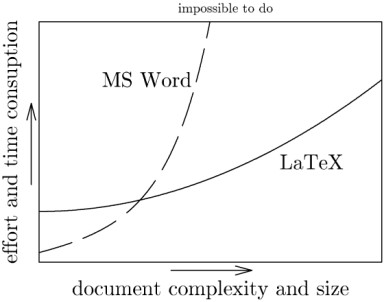
\includegraphics[width=\textwidth]{capitulo-ej/graphics/ejemplo-1.jpg}
            \caption{Subfigura 1.}
    \end{subfigure}
    ~~~~
    \begin{subfigure}[b]{0.45\textwidth}
            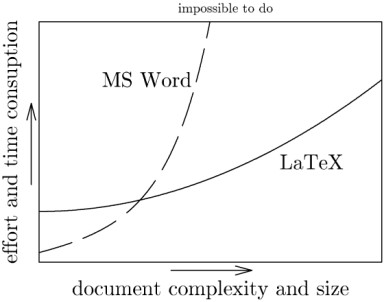
\includegraphics[width=\textwidth]{capitulo-ej/graphics/ejemplo-1.jpg}
            \caption{Subfigura 2.}

    \end{subfigure}
    \begin{subfigure}[b]{0.45\textwidth}
            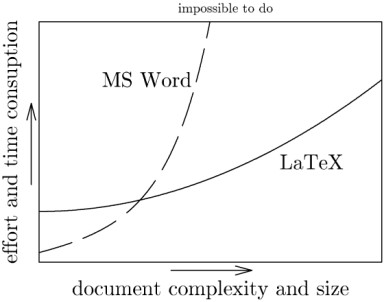
\includegraphics[width=\textwidth]{capitulo-ej/graphics/ejemplo-1.jpg}
            \caption{Subfigura 3.}
    \end{subfigure}
    ~~~~
    \begin{subfigure}[b]{0.45\textwidth}
            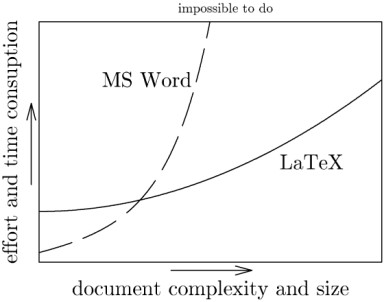
\includegraphics[width=\textwidth]{capitulo-ej/graphics/ejemplo-1.jpg}
            \caption{Subfigura 4.}

    \end{subfigure}
    \caption{\label{fig:ejemplo-fig-grilla}Ejemplo de una grilla de figuras en LaTex.}

\end{figure}

\subsection{Tablas}
Ejemplo de como hacer tablas utilizando el paquete table\footnote{http://en.wikibooks.org/wiki/LaTeX/Tables} de LaTex.
\begin{table}[!htpb]
    \begin{minipage}{\textwidth}
        \begin{center}
        \caption{\label{tab:tabla-ejemplo} Ejemplo de una tabla en LaTex.}
        \begin{tabular}{p{3cm} c c c c}
            \hline\\
            Año & Periodo & Columna & Columna2 & Columna3\\
            \hline
            \hline\\
            2014 & 29-12-13 / 31-05-14 & 10541 & 1052 & 2\\
            2013 & 30-12-12 / 21-12-13 & 153793 & 131306 & 70\\
            2012 & 01-01-12 / 22-12-12 & 37815 & 30588 & 11\\
            2011 & 03-01-11 / 29-12-11 & 53397 & 42264 & 62\\
            2010 & 11-10-09 / 25-12-10 & 21951 & 13760 & --$^a$\\
        \end{tabular}
        \footnotetext[1]{Esta es una nota.}
        \end{center}
    \end{minipage}
\end{table}

\subsection{Algoritmos}
Ejemplo de como hacer agloritmos utilizando el paquete algorithm\footnote{http://en.wikibooks.org/wiki/LaTeX/Algorithms} de LaTex.
\begin{algorithm}                      % enter the algorithm environment
\caption{Calculate $y = x^n$}          % give the algorithm a caption
\label{alg:alg1}                       % and a label for \ref{} commands later in the document
\begin{algorithmic}                    % enter the algorithmic environment
    \REQUIRE $n \geq 0 \vee x \neq 0$
    \ENSURE $y = x^n$
    \STATE $y \Leftarrow 1$
    \IF{$n < 0$}
        \STATE $X \Leftarrow 1 / x$
        \STATE $N \Leftarrow -n$
    \ELSE
        \STATE $X \Leftarrow x$
        \STATE $N \Leftarrow n$
    \ENDIF
    \WHILE{$N \neq 0$}
        \IF{$N$ is even}
            \STATE $X \Leftarrow X \times X$
            \STATE $N \Leftarrow N / 2$
        \ELSE[$N$ is odd]
            \STATE $y \Leftarrow y \times X$
            \STATE $N \Leftarrow N - 1$
        \ENDIF
    \ENDWHILE
\end{algorithmic}
\end{algorithm}

\subsection{Ecuaciones}
En esta sección se añade una pequeña ecuación con el fin de ejemplificar su
uso \addsymbol{symbol:x} \addsymbol{symbol:a_i}.
\begin{equation}\label{eq:ecuacion-ej}
  x = a_0 + \cfrac{1}{a_1
          + \cfrac{1}{a_2
          + \cfrac{1}{a_3 + \cfrac{1}{a_4} } } }
\end{equation}

\section{Referencias y citaciones}
Para referenciar secciones, figuras, tablas, algoritmos, o formulas se puede
emplear $\setminus$ref\{label-del-item\} o emplear cualquiera de las sigientes macros:


\begin{itemize}
\item $\setminus$secref\{label-sec\} : Ejemplo \secref{sec:figuras-tablas-algoritmos}
\item $\setminus$tabref\{label-tab\} : Ejemplo \tabref{tab:tabla-ejemplo}
\item $\setminus$figref\{label-fig\} : Ejemplo \figref{fig:ejemplo-fig-grilla}
\item $\setminus$algref\{label-alg\} : Ejemplo \algref{alg:alg1}
\item $\setminus$eqref\{label-eq\} : Ejemplo \eqref{eq:ecuacion-ej}
\end{itemize}

En esta sección se añade un ejemplo de como citar a un autor, utilizando
el $\setminus$cite\{label-bib1\} de bibText \footnote{http://en.wikibooks.org/wiki/LaTeX/Bibliography\_Management}.
Por ejemplo esta es una citación \cite{griffiths1997learning} a un solo
autor, y esta es a 2 autores \cite{griffiths1997learning, lamport1985i1}.

%\include{capitulo-3/capitulo-3}
%\include{capitulo-2/capitulo-2}
%\include{capitulo-4/capitulo-4}
%\include{capitulo-5/capitulo-5}
%\include{capitulo-6/capitulo-6}
%\include{capitulo-7/capitulo-7}

\appendix   % inician los apendices de tu tesis
% los cap'itulos que incluyas a partir de aqu'i aparecen
% como ap'endices
%\include{anexos/anexo-1}
% estos comandos generan la bilbiograf'ia
\printbibliography

\end{document}
